\subsection{Architecture du nouveau système}

La solution de création d'un nouveau SoC est une solution qui paraissait réaliste. Un projet avait déjà été commencé par \textit{G33KatWork} sur \href{https://github.com}{GitHub}. Ce projet était le début d'un système pour plusieurs plateformes dont la \nexys{}. Le projet comportait déjà un coeur LatticeMico32, de la RAM, un contrôleur UART, deux timers, un GPIO, le tout interfacé en Wishbone grâce à un connecteur \textit{Conbus} adapté, visible dans la figure \ref{new-system}.\\
Ceci a donc fourni la partie hardware minimale pour travailler mais aucun système logiciel ne l'accompagnait. Il fallait alors développer un firmware qui le ferait fonctionner.

\begin{figure}[h!]
\centering
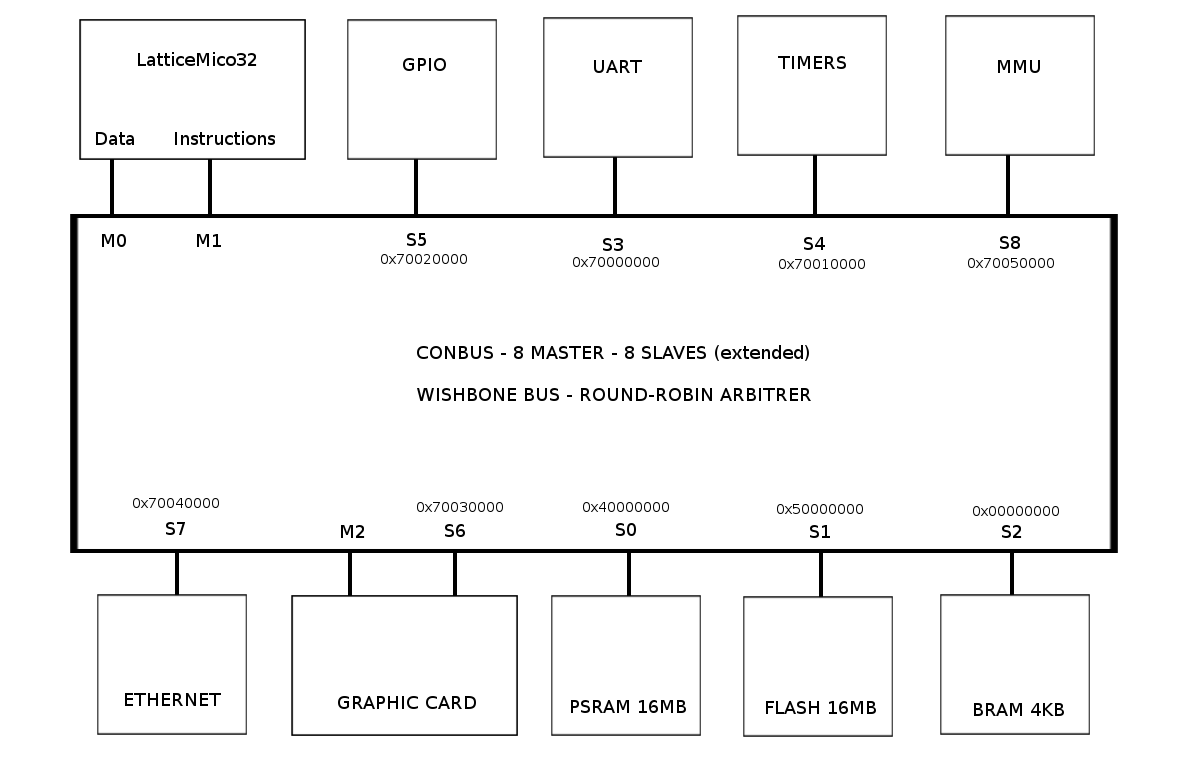
\includegraphics[scale=0.35]{general_system.png}
\caption{Schéma de l'architecture du nouveau système}
\label{new-system}
\end{figure}

\subsection{Le \english{bootloader}}

La premier programme réalisé a été le \english{bootloader} qui permet de charger en RAM un code par le biais de l'UART. Ce \english{bootloader} est implanté directement dans une RAM de 4096 octets réalisée en HDL. Le code du \english{bootloader} ne compte que quelques octets une fois compilé et s'exécute à chaque \english{reset} du processeur.\\
Ce logiciel, développé en \languagetoto{C} et appelé INSAFirmware, accueille l'utilisateur et se met en attente d'un fichier sur l'UART.\\
L'utilisateur doit alors envoyé 4 octets représentants la taille du fichier à lire par l'UART, les 4 octets suivant permettent de définir l'adresse où sera stocké le fichier. En général, ce code sera stocké en RAM. Finalement, l'utilisateur peut commencer à envoyer octet par octet son programme. Une fois le programme chargé, le firmware saute à l'adresse fournie par l'utilisateur et commence à exécuter le code.

\subsection{Création de nouveaux modules}

\subsubsection{Module Flash}

Pour compléter le système, le code Verilog du contrôleur de mémoire flash de \textit{Milkymist} a été récupéré et adapté sur le nouveau système. Il a ensuite fallu créer un driver qui permet de lire et d'écrire dans cette mémoire non volatile car son interface de contrôle fonctionne par commandes. Il faut écrire un octet de commande pour que la mémoire effectue la commande associée.\\
Il est actuellement possible d'écrire et lire des mots de 16 bits.

\subsubsection{Carte graphique}

La création d'une carte graphique a été entreprise. Elle comprend la gestion de la mémoire vidéo et l'affichage sur un moniteur connecté en VGA. Le schéma général de la carte graphique est présenté en figure \ref{carte-graphique}.

\begin{figure}[h!]
\centering
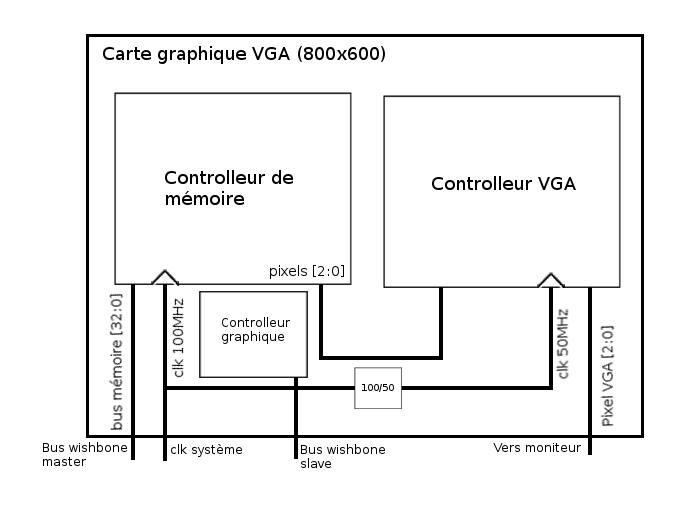
\includegraphics[scale=0.5]{vga.png}
\caption{Schéma de la carte graphique}
\label{carte-graphique}
\end{figure}

Cette carte graphique est reliée au bus Wishbone en tant qu'esclave grâce au contrôleur graphique qui permet de sélectionner l'adresse de base de la mémoire vidéo et d'activer ou de désactiver la carte graphique.\\
L'interface Wishbone maître sert à envoyer les requêtes mémoire pour acquérir les pixels du moniteur. De cette façon le contrôleur de mémoire s'exécute en parallèle du processeur. Il n'y aura pas d'accès mémoire concurrents puisque le \textit{Conbus} suit une stratégie \english{round-robin} pour la prise du bus.\\

Le contrôleur VGA actuellement implémenté dans la carte, ne permet d'afficher qu'une résolution de 800x600 mais pourrait facilement être modifié pour rendre possible le paramétrage dynamique de la résolution. Ainsi, on pourrait changer la résolution au niveau logiciel.\\
L'une des grandes problématiques est que la RAM embarquée sur la \nexys{} n'est pas assez rapide pour être lue à la fréquence de rafraichissement de l'écran. Il a donc fallu implémenter un système de bufferisation dans le contrôleur de mémoire. Celui-ci affiche $N$ pixels puis utilise les $3*N$ pixels suivant pour bufferiser les $N$ pixels qui suivront. On divise ainsi la fréquence d'affichage par quatre mais on obtient un affichage complet de l'écran. Cette manière de procéder fonctionne aussi pour des résolutions différentes.\\

À l'heure actuelle, la carte graphique n'est pas fonctionnelle mais est en bonne voie pour le devenir. La RAM de la \nexys{} fournit un moyen de lire un mot de 16 bits à chaque \english{tick} d'horloge système (100MHz) pendant 16 \english{ticks}. C'est ce qu'on appelle un \english{page mode}. On lit plusieurs valeurs à la suite sans attendre le temps de rafraîchissement de cette valeur comme dans un \english{single-read mode} où une seule valeur est lue à la fois. Cette fonctionnalité est en train d'être ajoutée au niveau matériel au contrôleur de PSRAM afin de gérer ce mode et ainsi d'accélérer la bufferisation pour essayer de passer à un taux de rafraîchissement seulement divisé par deux.\\

Il n'existe sur la \nexys{} qu'une mémoire capable d'être lue à la volée à la fréquence demandée : la flash avec interface SPI en \english{quad mode}. SPI est un protocole créé par des entreprises pour effectuer des communications série, c'est-à-dire qu'il ne faut qu'un seul \textit{pin} de données pour communiquer avec le périphérique. Cette flash a en plus un \english{quad mode} qui permet de lire 4 bits à chaque \english{tick} d'horloge, ceci permet de multiplier le débit par quatre. Dans ce mode, la fréquence maximale de fonctionnement est la même que celle du VGA (50MHz). En arrivant à l'interfacer, nous pourrions alors tenter d'afficher des images sans bufferisation mais une mémoire flash est beaucoup plus sensible aux cycles d'écritures et vieillit plus vite qu'une RAM.

\subsubsection{\english{Memory Management Unit}}

Une MMU est un composant qui permet de faire une translation d'adresse entre espace virtuel et espace physique. Cette MMU très simple pourrait permettre d'implémenter un fonctionnement multi-tâches tel qu'il est fait sur les ordinateurs classiques. La translation d'adresses est illustrée dans la figure \ref{memory-management-unit-translation}.

\begin{figure}[h!]
\centering
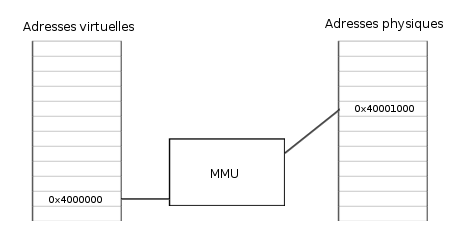
\includegraphics[scale=0.6]{mmu_translation.png}
\caption{Schéma d'une translation d'adresses virtuelles à physiques}
\label{memory-management-unit-translation}
\end{figure}

Ce module Verilog coupe le bus d'adresse du LatticeMico32 pour faire la translation. Il a une interface esclave connectée au bus Wishbone qui lui permet d'être paramétré. Cette MMU est illustrée à la figure \ref{memory-management-unit}.\\
Son fonctionnement est simple, on peut l'activer ou la désactiver en écrivant dans le registre de contrôle. Lorsqu'elle est désactivée, il n'y a pas de translation d'adresse, c'est-à-dire que l'adresse physique est égale à l'adresse virtuelle. Si elle est activée, elle
utilise un deuxième registre qui stocke la valeur de l'\english{offset} à ajouter à l'adresse virtuelle. Ainsi, si l'adresse en entrée (l'adresse virtuelle) est de 0x40000000 et que l'\english{offset} de la MMU est 0x1000, l'adresse physique sera 0x40001000.

\begin{figure}[h!]
\centering
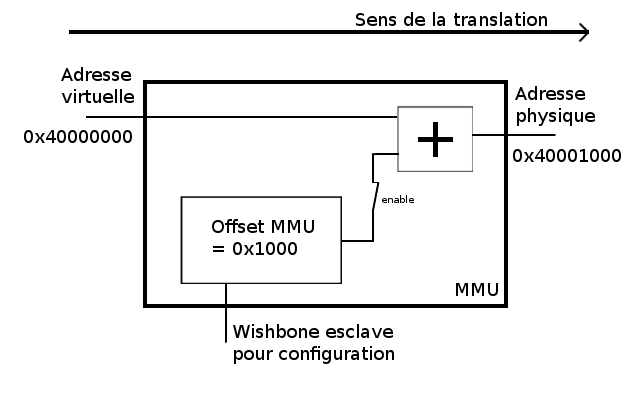
\includegraphics[scale=0.5]{mmu.png}
\caption{Schéma de la MMU}
\label{memory-management-unit}
\end{figure}

\subsubsection{Module Ethernet}

Nous avons trouvé un module Ethernet sur un \href{http://svn.ohwr.org/lm32/cores/mac/rtl/}{SVN}. Il s'agissait du même module que celui proposé sur \href{http://opencores.org/project,ethmac}{OpenCores}. Ce module a une interface de bus Wishbone, il avait été utilisé précédemment dans un système avec un LM32. L'idée est de pouvoir relier deux cartes avec un câble Ethernet et d'utiliser cette interface de communication afin d'échanger des données. Cette interface nous offre des services de base (CRC, accès au medium CSMA/CD) pour envoyer des données de manière à résister à des accès simultanés au medium et des erreurs de transmission dues aux interférences.\\

Nous avons également trouvé le driver de ce module sur le même \href{http://svn.ohwr.org/lm32/crt/mac/}{SVN}. Cependant, pour que ce driver soit fonctionnel, il faudrait connecter l'interruption au processeur, puis gérer l'interruption associée dans le kernel.
